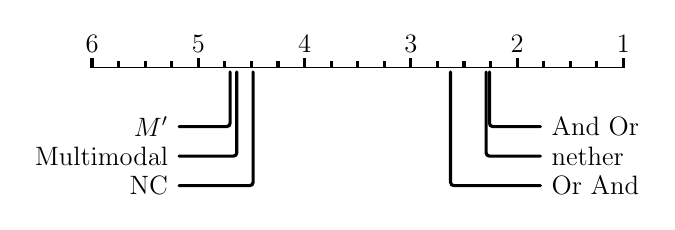
\begin{tikzpicture}[
  treatment line/.style={rounded corners=1.5pt, line cap=round, shorten >=1pt, line width=.5mm},
  treatment label/.style={font=\large},
  group line/.style={ultra thick},
  scale={0.8},
]

\begin{axis}[
  clip={false},
  axis x line={center},
  axis y line={none},
  axis line style={-},
  xmin={1},
  ymax={0},
  scale only axis={true},
  width={\axisdefaultwidth},
  ticklabel style={anchor=south, yshift=1.3*\pgfkeysvalueof{/pgfplots/major tick length}, font=\large},
  every tick/.style={draw=black, line width=.5mm},
  major tick style={yshift=.5*\pgfkeysvalueof{/pgfplots/major tick length}},
  minor tick style={yshift=.5*\pgfkeysvalueof{/pgfplots/minor tick length}},
  title style={yshift=\baselineskip},
  xmax={6},
  ymin={-4.5},
  height={5\baselineskip},
  xtick={1,2,3,4,5,6},
  minor x tick num={3},
  x dir={reverse},
]

\draw[treatment line] ([yshift=-2pt] axis cs:2.2598425196850394, 0) |- (axis cs:1.7598425196850394, -2.0)
  node[treatment label, anchor=west] {And Or};
\draw[treatment line] ([yshift=-2pt] axis cs:2.2913385826771653, 0) |- (axis cs:1.7598425196850394, -3.0)
  node[treatment label, anchor=west] {nether};
\draw[treatment line] ([yshift=-2pt] axis cs:2.625984251968504, 0) |- (axis cs:1.7598425196850394, -4.0)
  node[treatment label, anchor=west] {Or And};
\draw[treatment line] ([yshift=-2pt] axis cs:4.484251968503937, 0) |- (axis cs:5.200787401574803, -4.0)
  node[treatment label, anchor=east] {NC};
\draw[treatment line] ([yshift=-2pt] axis cs:4.637795275590551, 0) |- (axis cs:5.200787401574803, -3.0)
  node[treatment label, anchor=east] {Multimodal};
\draw[treatment line] ([yshift=-2pt] axis cs:4.700787401574803, 0) |- (axis cs:5.200787401574803, -2.0)
  node[treatment label, anchor=east] {$M'$};

\end{axis}
\end{tikzpicture}